\section{Editor, Visualization, and Playback}\label{sec:editor-visualization}

The editor uses Monaco because it provides language registration, tokenization, themes, keyboard actions, and marker
support in a browser editor widget~\cite{Microsoft_Monaco_2026}.
Motivo Studio registers a Motivo language identifier and a Monarch tokenizer for language keywords, instruments, drum
notes, note literals, comments, and operators.
When compilation fails, diagnostics are converted into markers so the source location is visible inside the editor
rather than only in a log panel.

\subsection{IDE Integration and Diagnostics}\label{detail-subsec:ide-integration-and-diagnostics}

The playground features an IDE-like experience powered by the Monaco Editor.
A custom ``Monarch'' tokenizer was implemented for Motivo to provide syntax highlighting for musical keywords, pitch
literals, and control flow.

The most significant integration is the \textit{Diagnostics Feedback Loop}.
When a compilation fails, the Express server parses the structured error output from the compiler and returns it to the
client.
The React application then converts these diagnostics into Monaco ``Markers'', which underline the erroneous code and
display the compiler's semantic or syntax error messages in a tooltip.
This real-time feedback is enabled by the fast local compilation times discussed in the evaluation chapter.

The piano roll exists because MIDI is symbolic.
A successful compile response is not audio; it is a binary event file.
The browser parses that MIDI data and renders note events as colored rectangles against a piano-style vertical scale and
a horizontal time axis.
This view gives the user a visual check on timing, density, and pitch range before listening.
The playback layer uses browser audio libraries and SoundFont-based instruments to audition the
result~\cite{ToneJS_2026,SoundFontPlayer_2026}.
The rendered view and playback controls make Motivo Studio a practical development surface for the compiler.

\subsection{The Piano Roll and Synthesis}\label{detail-subsec:the-piano-roll-and-synthesis}

To visualize the composition, a custom \textit{Piano Roll} component was built using the HTML5 Canvas API\@.
Upon a successful compilation, the browser parses the returned MIDI bytes and renders them as colored rectangles on a
scrolling timeline.

The synthesis engine utilizes the \textit{Tone.js} library.
Because MIDI files contain only instructions and no sound, the playground loads a set of high-quality
\textit{Soundfonts} representing General MIDI instruments.
The playback logic schedules notes in the browser's audio context, allowing the user to hear their ``coded'' composition
instantly.
The synchronization between the scrolling piano roll and the audio playback is maintained through a high-precision
request-animation-frame loop, ensuring a professional and ``alive'' feel to the prototype.

\begin{figure}[p]
  \centering
  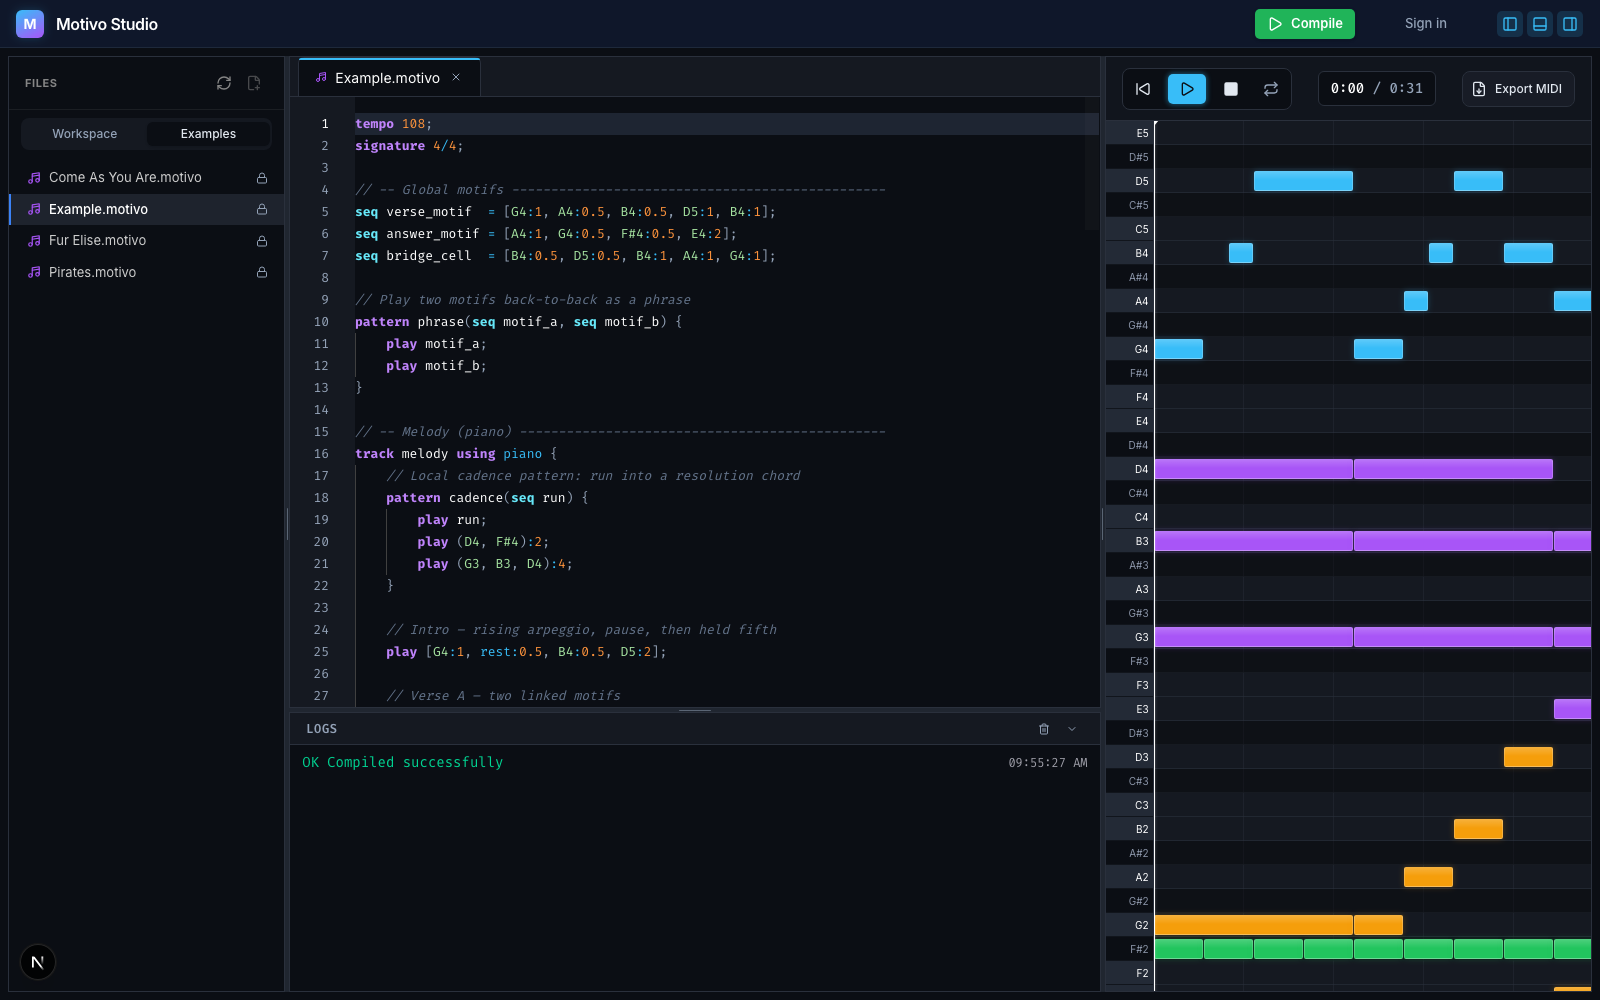
\includegraphics[width=\textwidth]{assets/screenshots/motivo-studio-success.png}
  \caption{Motivo Studio after a successful local compile.
    The screenshot shows the Monaco editor, success log, playback controls, and generated piano-roll
    visualization for the
  default Motivo snippet.}\label{fig:studio-success-screenshot}
\end{figure}

\begin{figure}[htbp]
  \centering
  \begin{tikzpicture}[
      panel/.style={rounded corners=4pt, draw=motivoInk!55, very thick, align=center, font=\small\sffamily},
      small/.style={font=\scriptsize\sffamily, text=motivoInk}
    ]
    \node[panel, fill=motivoInk!6, minimum width=12.5cm, minimum height=7.0cm] (shell) {};
    \node[panel, fill=motivoBlue!12, minimum width=5.7cm, minimum height=5.8cm, anchor=west] at (-5.9,0)
    {Monaco editor\\Motivo source};
    \node[panel, fill=motivoGreen!12, minimum width=5.7cm, minimum height=3.6cm, anchor=east] at (5.9,1.1)
    {Piano-roll canvas\\generated notes};
    \node[panel, fill=motivoAmber!18, minimum width=5.7cm, minimum height=1.7cm, anchor=east] at (5.9,-2.4)
    {Playback bar\\transport, progress, download};
    \node[panel, fill=motivoRose!12, minimum width=12.2cm, minimum height=0.75cm, anchor=south] at (0,-3.25)
    {Diagnostics and logs};

    \foreach \x/\w/\c in {-4.7/0.8/motivoBlue,-3.8/1.2/motivoCyan,-2.5/1.0/motivoGreen,-1.4/1.5/motivoAmber} {
      \draw[fill=\c!70, draw=white] (\x,1.8) rectangle ++(\w,0.22);
      \draw[fill=\c!70, draw=white] (\x+0.4,1.2) rectangle ++(\w,0.22);
      \draw[fill=\c!70, draw=white] (\x+0.1,0.6) rectangle ++(\w,0.22);
    }
    \draw[fill=motivoBlue!70, draw=white] (1.2,2.1) rectangle ++(1.0,0.26);
    \draw[fill=motivoGreen!70, draw=white] (2.5,1.5) rectangle ++(0.7,0.26);
    \draw[fill=motivoAmber!70, draw=white] (3.6,0.9) rectangle ++(1.3,0.26);
    \draw[fill=motivoRose!70, draw=white] (4.9,2.4) rectangle ++(0.9,0.26);
    \draw[fill=motivoViolet!70, draw=white] (2.0,0.3) rectangle ++(2.0,0.26);
    \node[small] at (-0.1,3.15) {Motivo Studio workspace layout};
  \end{tikzpicture}
  \caption{Motivo Studio workspace organization.
    The figure summarizes the editor, visualization, playback, and diagnostics surfaces implemented in the
  client.}\label{fig:studio-workspace}
\end{figure}
